\documentclass{article}

\usepackage{tikz}
\usepackage{tikz-qtree}
\tikzset{every tree node/.style={align=center, anchor=north}}
\usetikzlibrary{positioning}

\begin{document}

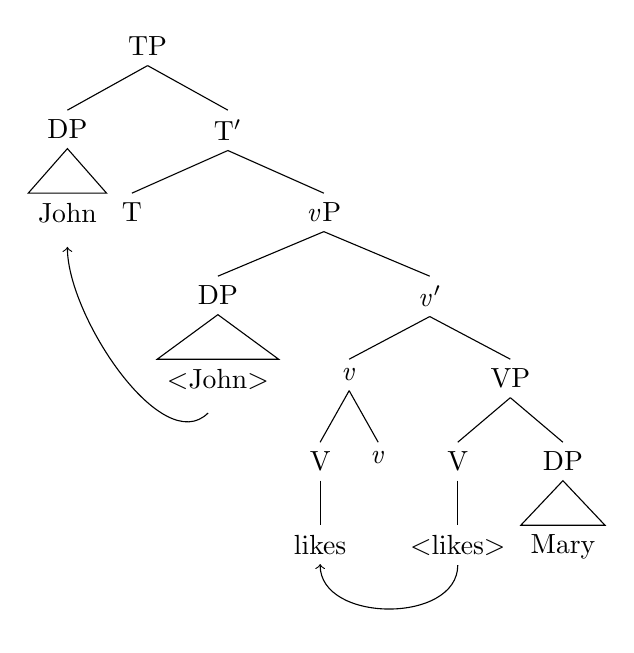
\begin{tikzpicture}
\Tree
[.TP
    [.\node(DP1-rel){DP}; \edge[roof]; {John} ]
    [.T$'$
        [.T ]
        [.\emph{v}P
            [.\node(DP2-rel){DP}; \edge[roof]; {$<$John$>$} ]
            [.\emph{v}$'$
                [.\emph{v}
                    [.V \node(V1){likes}; ]
                    [.\emph{v} ]
                ]
                [.VP
                    [.V \node(V2){$<$likes$>$}; ]
                    [.DP \edge[roof]; {Mary} ]
                ]
            ]
        ]
    ]
]
\node (DP1) [below=1cm of DP1-rel] {};
\node (DP2) [below=1cm of DP2-rel] {};
\draw[->] (DP2)..controls +(south west:1) and +(south:1)..(DP1);
\draw[->] (V2)..controls +(south:1) and +(south:1)..(V1);
\end{tikzpicture}

\end{document}
